\section{ХОД РАБОТЫ}

\subsection{Постановка задачи}

В ходе данной лабораторной работы требуется выполнить проектирование
и реализацию небольшой семантической сети с использованием языка Пролог.

В качестве темы, определяющей набор объектов и отношений между ними,
выберем стихотворение Самуила Маршака <<Дом, который построил Джек>>.

\subsection{Проктирование семантической сети}

Приведем текст стихотворения --- основы семантической сети.

\begin{center}
С. Маршак \\
Дом, который построил Джек
\end{center}

\begin{verse}
Вот \textbf{дом}, \\
Который \textit{построил} \textbf{Джек}.

А это \textbf{пшеница}, \\
Которая в \texttt{темном} \textbf{чулане} \textit{хранится} \\
В \textbf{доме}, \\
Который \textit{построил} \textbf{Джек}.

А это \textit{веселая} \textbf{птица-синица}, \\
Которая часто \textit{ворует} \textbf{пшеницу}, \\
Которая в \texttt{темном} \textbf{чулане} \textit{хранится} \\
В \textbf{доме}, \\
Который \textit{построил} \textbf{Джек}.

Вот \textbf{кот}, \\
Который \textit{пугает} и \textit{ловит} \textbf{синицу}, \\
Которая часто \textit{ворует} \textbf{пшеницу}, \\
Которая в \texttt{темном} \textbf{чулане} \textit{хранится} \\
В \textbf{доме}, \\
Который \textit{построил} \textbf{Джек}.

Вот \textbf{пес} \texttt{без хвоста}, \\
Который за шиворот \textit{треплет} \textbf{кота}, \\
Который \textit{пугает} и \textit{ловит} \textbf{синицу}, \\
Которая часто \textit{ворует} \textbf{пшеницу}, \\
Которая в \texttt{темном} \textbf{чулане} \textit{хранится} \\
В \textbf{доме}, \\
Который \textit{построил} \textbf{Джек}.

А это \textbf{корова} \texttt{безрогая}, \\
\textit{Лягнувшая} \texttt{старого} \textbf{пса} \texttt{без хвоста}, \\
Который за шиворот \textit{треплет} \textbf{кота}, \\
Который \textit{пугает} и \textit{ловит} \textbf{синицу}, \\
Которая часто \textit{ворует} \textbf{пшеницу}, \\
Которая в \texttt{темном} \textbf{чулане} \textit{хранится} \\
В \textbf{доме}, \\
Который \textit{построил} \textbf{Джек}.

А это \textbf{старушка}, \texttt{седая} и \texttt{строгая}, \\
Которая \textit{доит} \textbf{корову} \texttt{безрогую}, \\
\textit{Лягнувшую} \texttt{старого} \textbf{пса} \texttt{без хвоста}, \\
Который за шиворот \textit{треплет} \textbf{кота}, \\
Который \textit{пугает} и \textit{ловит} \textbf{синицу}, \\
Которая часто \textit{ворует} \textbf{пшеницу}, \\
Которая в \texttt{темном} \textbf{чулане} \textit{хранится} \\
В \textbf{доме}, \\
Который \textit{построил} \textbf{Джек}.

А это \texttt{ленивый} и \texttt{толстый} \textbf{пастух}, \\
Который \textit{бранится} с \textbf{коровницей} \texttt{строгою}, \\
Которая \textit{доит} \textbf{корову} \texttt{безрогую}, \\
\textit{Лягнувшую} \texttt{старого} \textbf{пса} \texttt{без хвоста}, \\
Который за шиворот \textit{треплет} \textbf{кота}, \\
Который \textit{пугает} и \textit{ловит} \textbf{синицу}, \\
Которая часто \textit{ворует} \textbf{пшеницу}, \\
Которая в \texttt{темном} \textbf{чулане} \textit{хранится} \\
В \textbf{доме}, \\
Который \textit{построил} \textbf{Джек}.

Вот \textbf{два петуха}, \\
Которые \textit{будят} того \textbf{пастуха}, \\
Который \textit{бранится} с \textbf{коровницей} \texttt{строгою}, \\
Которая \textit{доит} \textbf{корову} \texttt{безрогую}, \\
\textit{Лягнувшую} \texttt{старого} \textbf{пса} \texttt{без хвоста}, \\
Который за шиворот \textit{треплет} \textbf{кота}, \\
Который \textit{пугает} и \textit{ловит} \textbf{синицу}, \\
Которая часто \textit{ворует} \textbf{пшеницу}, \\
Которая в \texttt{темном} \textbf{чулане} \textit{хранится} \\
В \textbf{доме}, \\
Который \textit{построил} \textbf{Джек}.
\end{verse}

Здесь объекты будущей сети выделены \textbf{жирным},
отношения между ними --- \textit{курсивом},
а свойства --- \texttt{моноширинным шрифтом}.


\subsection{Реализация семантической сети}

Приведем элепменты семантической сети к виду,
пригодному для использования в языке Пролог.
Для этого введем следующие предикаты:

\begin{itemize}
\item \texttt{who(X)} --- одушевленный объект;
\item \texttt{what(X)} --- неодушевленный объект;
\item \texttt{has\_prop(X)} --- свойство объекта;
\item \texttt{do(X)} --- отношение;
\item \texttt{how(X)} --- свойство отношения;
\end{itemize}

Заметим, что предикат \texttt{has\_prop(X)}
не являются непременно необходимым для построения сети,
а введен для краткости и удобства.

Имея в распоряжении вышеперечисленные предикаты,
а также служебные
\texttt{s(L)} (помещение фрагмента сети \texttt{L} в базу знаний) и
\texttt{m(X, L)} (проверка наличия элемента \texttt{X} в списке \texttt{L})
мы можем построить семантическую сеть стихотворения,
как показано на рисунке~\ref{lst:jack}.

\pagebreak

\lstinputlisting[style=source_code,numbers=left,numberstyle=\texttt,xleftmargin=2em,
                 caption=Представление семантической сети на языке Пролог,
                 language=prolog,label=lst:jack]{code/jack.pro}

\pagebreak

Приведем тестовые вопросы, которые были заданы разработанной базе знаний:

\begin{enumerate}
\item \textit{Где хранится пшеница в доме, который построил Джек?}

  Текст запроса на языке Пролог приведен на рисунке~\ref{lst:q_1}.

  \begin{lstlisting}[style=source_code,language=prolog,
    caption=Текст запроса,label=lst:q_1]
 q_1(X) :-
     s(S1), s(S2),
     m(what(house), S1),
     m(do(contain), S1),
     m(what(X), S1),
     m(what(X), S2),
     m(do(keep), S2),
     m(what(wheat), S2).
  \end{lstlisting}

  Результат выполнения запроса приведен на рисунке~\ref{fig:q}.

\item \textit{Кто бранится с тем, кто доит корову?}

  Текст запроса на языке Пролог приведен на рисунке~\ref{lst:q_2}.

  \begin{lstlisting}[style=source_code,language=prolog,
    caption=Текст запроса,label=lst:q_2]
 q_2(X, Y) :-
     s(S1), s(S2),
     m(who(X), S1),
     m(do(scold), S1),
     m(who(Y), S1),
     m(who(Y), S2),
     m(do(milk), S2),
     m(who(cow), S2).
  \end{lstlisting}

  Результат выполнения запроса приведен на рисунке~\ref{fig:q}.

\newpage

\item \textit{Как пес треплет того, кто ловит синицу?}

  Текст запроса на языке Пролог приведен на рисунке~\ref{lst:q_3}.

  \begin{lstlisting}[style=source_code,language=prolog,
    caption=Текст запроса,label=lst:q_3]
 q_3(X, Y) :-
     s(S1), s(S2),
     m(who(dog), S1),
     m(do(shake), S1),
     m(who(Y), S1),
     m(how(X), S1),
     m(who(Y), S2),
     m(do(catch), S2),
     m(who(titmouse), S2).
  \end{lstlisting}

  Результат выполнения запроса приведен на рисунке~\ref{fig:q}.

\item \textit{Кто пугает того, кто ворует пшеницу?}

  Текст запроса на языке Пролог приведен на рисунке~\ref{lst:q_4}.

  \begin{lstlisting}[style=source_code,language=prolog,
    caption=Текст запроса,label=lst:q_4]
 q_4(X, Y) :-
     s(S1), s(S2),
     m(who(X), S1),
     m(do(fright), S1),
     m(who(Y), S1),
     m(who(Y), S2),
     m(do(steal), S2),
     m(what(wheat), S2).
  \end{lstlisting}

  Результат выполнения запроса приведен на рисунке~\ref{fig:q}.

\newpage

\item \textit{Что хранится в чулане дома, который построил Джек?}

  Текст запроса на языке Пролог приведен на рисунке~\ref{lst:q_5}.

  \begin{lstlisting}[style=source_code,language=prolog,
    caption=Текст запроса,label=lst:q_5]
 q_5(X) :-
     s(S1), s(S2),
     m(what(house), S1),
     m(do(contain), S1),
     m(what(Y), S1),
     m(what(Y), S2),
     m(what(X), S2).
  \end{lstlisting}

  Результат выполнения запроса приведен на рисунке~\ref{fig:q}.

\item \textit{Кто треплет того, кто ловит синицу?}

  Текст запроса на языке Пролог приведен на рисунке~\ref{lst:q_6}.

  \begin{lstlisting}[style=source_code,language=prolog,
    caption=Текст запроса,label=lst:q_6]
 q_6(X, Y) :-
     s(S1), s(S2),
     m(who(X), S1),
     m(do(shake), S1),
     m(who(Y), S1),
     m(who(Y), S2),
     m(do(catch), S2),
     m(who(titmouse), S2).
  \end{lstlisting}

  Результат выполнения запроса приведен на рисунке~\ref{fig:q}.

\newpage

\item \textit{Кто ворует то, что в темном чулане хранится?}

  Текст запроса на языке Пролог приведен на рисунке~\ref{lst:q_7}.

  \begin{lstlisting}[style=source_code,language=prolog,
    caption=Текст запроса,label=lst:q_7]
 q_7(X, Y) :-
     s(S1), s(S2),
     m(who(X), S1),
     m(do(steal), S1),
     m(what(Y), S1),
     m(what(lumber-room), S2),
     m(do(keep), S2),
     m(what(Y), S2).
  \end{lstlisting}

  Результат выполнения запроса приведен на рисунке~\ref{fig:q}.

\end{enumerate}

\begin{figure}[h!]
  \centering
  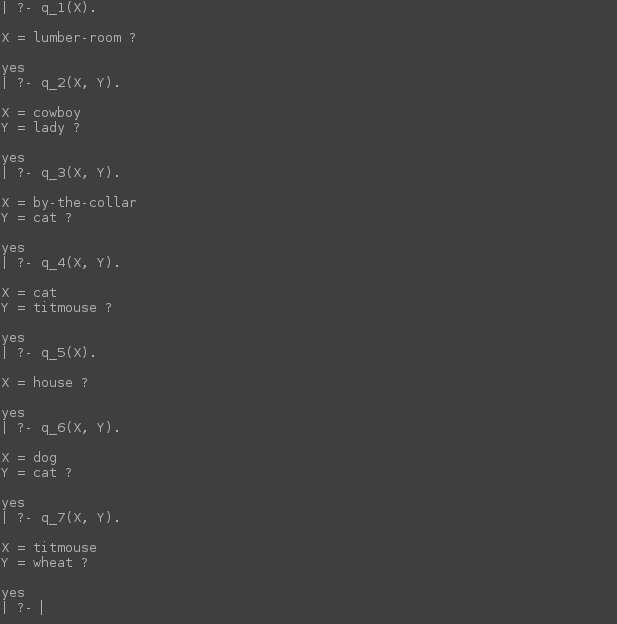
\includegraphics[width=130mm]{img/q}
  \caption{Результат выполнения запроса}
  \label{fig:q}
\end{figure}

\newpage